\documentclass[
11pt, % The default document font size, options: 10pt, 11pt, 12pt
%codirector, % Uncomment to add a codirector to the title page
]{charter} 




% El títulos de la memoria, se usa en la carátula y se puede usar el cualquier lugar del documento con el comando \ttitle
\titulo{Sistema de Iluminación y  Riego por Goteo} 

% Nombre del posgrado, se usa en la carátula y se puede usar el cualquier lugar del documento con el comando \degreename
\posgrado{Carrera de Especialización en Sistemas Embebidos} 
%\posgrado{Carrera de Especialización en Internet de las Cosas} 
%\posgrado{Carrera de Especialización en Intelegencia Artificial}
%\posgrado{Maestría en Sistemas Embebidos} 
%\posgrado{Maestría en Internet de las cosas}

% Tu nombre, se puede usar el cualquier lugar del documento con el comando \authorname
\autor{Ing. Escribá Pedro Santiago} 

% El nombre del director y co-director, se puede usar el cualquier lugar del documento con el comando \supname y \cosupname y \pertesupname y \pertecosupname
\director{Ing. Esp. Brignone Matias Nicolás}
\pertenenciaDirector{Encora} 
% FIXME:NO IMPLEMENTADO EL CODIRECTOR ni su pertenencia
\codirector{John Doe} % para que aparezca en la portada se debe descomentar la opción codirector en el documentclass
\pertenenciaCoDirector{FIUBA}

% Nombre del cliente, quien va a aprobar los resultados del proyecto, se puede usar con el comando \clientename y \empclientename
\cliente{Ing. Rodrigo Fernandez Frittelli}
\empresaCliente{RiegoTec}

% Nombre y pertenencia de los jurados, se pueden usar el cualquier lugar del documento con el comando \jurunoname, \jurdosname y \jurtresname y \perteunoname, \pertedosname y \pertetresname.
\juradoUno{Nombre y Apellido (1)}
\pertenenciaJurUno{pertenencia (1)} 
\juradoDos{Nombre y Apellido (2)}
\pertenenciaJurDos{pertenencia (2)}
\juradoTres{Nombre y Apellido (3)}
\pertenenciaJurTres{pertenencia (3)}
 
\fechaINICIO{20 de octubre de 2022}		%Fecha de inicio de la cursada de GdP \fechaInicioName
\fechaFINALPlan{8 de diciembre de 2022} 	%Fecha de final de cursada de GdP
\fechaFINALTrabajo{15 de Agosto de 2022}	%Fecha de defensa pública del trabajo final


\begin{document}

\maketitle
\thispagestyle{empty}
\pagebreak


\thispagestyle{empty}
{\setlength{\parskip}{0pt}
\tableofcontents{}
}
\pagebreak


\section*{Registros de cambios}
\label{sec:registro}


\begin{table}[ht]
\label{tab:registro}
\centering
\begin{tabularx}{\linewidth}{@{}|c|X|c|@{}}
\hline
\rowcolor[HTML]{C0C0C0} 
Revisión & \multicolumn{1}{c|}{\cellcolor[HTML]{C0C0C0}Detalles de los cambios realizados} & Fecha      \\ \hline
0      & Creación del documento                                 &\fechaInicioName \\ \hline
1      & Se completa hasta el punto 5 inclusive                 & 03/11/2022 \\ \hline
%2      & Se completa hasta el punto 7 inclusive
%		  Se puede agregar algo más \newline
%		  En distintas líneas \newline
%		  Así                                                    & dd/mm/aaaa \\ \hline
%3      & Se completa hasta el punto 11 inclusive                & dd/mm/aaaa \\ \hline
%4      & Se completa el plan	                                 & dd/mm/aaaa \\ \hline
\end{tabularx}
\end{table}

\pagebreak



\section*{Acta de constitución del proyecto}
\label{sec:acta}

\begin{flushright}
Buenos Aires, \fechaInicioName
\end{flushright}

\vspace{2cm}

Por medio de la presente se acuerda con el Ing. \authorname\hspace{1px} que su Trabajo Final de la \degreename\hspace{1px} se titulará ``\ttitle'', consistirá esencialmente en la implementación de un prototipo de un sistema de riego por goteo, y tendrá un presupuesto preliminar estimado de 70 hs de trabajo y ARS 10000, con fecha de inicio \fechaInicioName\hspace{1px} y fecha de presentación pública \fechaFinalName.

Se adjunta a esta acta la planificación inicial.

\vfill

% Esta parte se construye sola con la información que hayan cargado en el preámbulo del documento y no debe modificarla
\begin{table}[ht]
\centering
\begin{tabular}{ccc}
\begin{tabular}[c]{@{}c@{}}Ariel Lutenberg \\ Director posgrado FIUBA\end{tabular} & \hspace{2cm} & \begin{tabular}[c]{@{}c@{}}\clientename \\ \empclientename \end{tabular} \vspace{2.5cm} \\ 
\multicolumn{3}{c}{\begin{tabular}[c]{@{}c@{}} \supname \\ Director del Trabajo Final\end{tabular}} \vspace{2.5cm} \\
%\begin{tabular}[c]{@{}c@{}}\jurunoname \\ Jurado del Trabajo Final\end{tabular}     &  & \begin{tabular}[c]{@{}c@{}}\jurdosname\\ Jurado del Trabajo Final\end{tabular}  \vspace{2.5cm}  \\
%\multicolumn{3}{c}{\begin{tabular}[c]{@{}c@{}} \jurtresname\\ Jurado del Trabajo Final\end{tabular}} \vspace{.5cm}                                                                     
\end{tabular}
\end{table}




\section{1. Descripción técnica-conceptual del proyecto a realizar}
\label{sec:descripcion}

Con el objetivo de aprender nuevas tecnologías y aplicar y arraigar los conocimientos adquiridos en la especialidad de Sistemas Embebidos de la UBA es que se propone el presente proyecto. Este busca implementar nuevas tecnologías a los sistemas de riegos actuales con el propósito de garantizar un cultivo de excelencia, donde el grado de impacto negativo de las variables climáticas sean lo menor posible. En complemento, se propone también suministrar un sistema de iluminación moderno y vistoso. 

De esta manera, surgen una gran variedad de soluciones tecnológicas siendo imperioso seleccionar la que mejor se adapte a satisfacer esta necesidad. Por ello es que se propone utilizar uno o más sensores de humedad por cada cultivo y, mediante un lazo de control cerrado, suministrar el agua que sea requerida. La información para cada especie de planta se encontrará en un servidor virtual y mismo enviará la información al sistema embebido por WI-FI.

A diferencia de otros sistemas de riego, el presente incorpora nuevas tecnologías de comunicación y una interfaz de usuario. Es así que cualquier persona con un SmarthPhone podrá configurar el cultivo asociado a un sensor y obtener estadísticas de la humedad de la tierra. También controlará un arreglo de LEDs RGB situado cercano a un sensor o plantín.

En la Figura \ref{fig:diagBloques} se puede observar los diferentes bloques del proyecto, seccionado de acuerdo a las tecnologías a utilizar. La interfaz de usuario abarca el high level tecnológico y más cercano a la persona, mientras que el sistema embebido representa el low level tecnológico y más lejano a la persona.

\begin{figure}[htpb]
\centering 
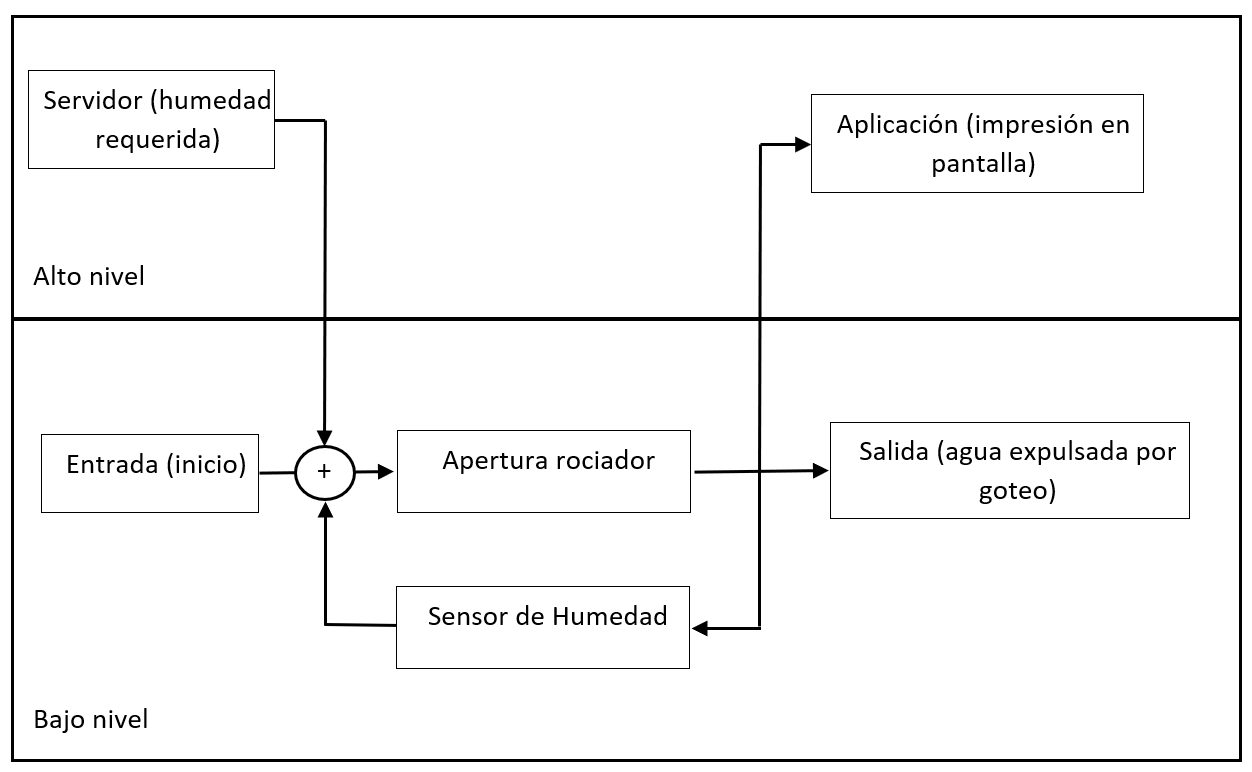
\includegraphics[width=1\textwidth]{./Figuras/digBloq.png}
\caption{Diagrama en bloques del sistema}
\label{fig:diagBloques}
\end{figure}


\section{2. Identificación y análisis de los interesados}
\label{sec:interesados}

En esta sección se estudian los interesados en el proyecto. En la Tabla \ref{tab:interesados} se puede apreciar los distintos roles, organización y puesto de las personas que poseen un cierto interés en el producto a desarrollar.

\begin{table}[ht]
%\caption{Identificación de los interesados}
%\label{tab:interesados}
\begin{tabularx}{\linewidth}{@{}|l|X|X|l|@{}}
\hline
\rowcolor[HTML]{C0C0C0} 
Rol           & Nombre y Apellido & Organización 	& Puesto 	\\ \hline
Auspiciante   & \clientename      &\empclientename 	& -        	\\ \hline
Cliente       & \clientename      &\empclientename	& -      	\\ \hline
Responsable   & \authorname       & FIUBA        	& Alumno 	\\ \hline
Orientador    & \supname	      & \pertesupname 	& Director Trabajo final \\ \hline
Usuario final & Ana Fernandez     &Particular    	& -       	\\ \hline
\end{tabularx}
\caption{Interesados}
\label{tab:interesados}
\end{table}

\begin{itemize}
	\item Auspiciante y Cliente: es riguroso y exigente. Desea un producto final en condiciones óptimas y sin fallas.
	\item Orientador: Matías es un profesional de excelencia, capaz de asistir en las necesidades que surjan.
	\item Usuario final: profesional de herbología.
\end{itemize}



\section{3. Propósito del proyecto}
\label{sec:proposito}

El propósito de este proyecto es diseñar un prototipo funcional capaz de administrar agua mediante la tecnología de goteo a un cultivo determinado, satisfaciendo las necesidades del cliente involucrado. A su vez, se pretende aplicar los conocimientos adquiridos en la carrera de especialización de Sistemas Embebidos permitiendo que los mismos sean afianzados.


\section{4. Alcance del proyecto}
\label{sec:alcance}

Acorde a las necesidades del cliente, el proyecto incluye el desarrollo de un firmware en lenguaje C encargado del control a lazo cerrado del sistema de riego y su comunicación con un servidor. También es parte de este proyecto el desarrollo mecánico de un prototipo funcional de riego por goteo que responda a las necesidades de un único cultivo. Además se incluye el código para el control del sistema de iluminación y su desarrollo físico y, por último, una demo de una interfaz de usuario para utilizar en SmartPhones.

En cambio, no es parte de este proyecto el desarrollo del código de la interfaz de usuario y brindar soporte a la misma. Tampoco se incluye el desarrollo de un PBC para alojar los diferentes componentes ni el desarrollo del hardware necesario.


\section{5. Supuestos del proyecto}
\label{sec:supuestos}

Para el desarrollo del presente proyecto se supone que:

\begin{itemize}
	\item Se conocen todos los conceptos técnicos necesarios para su desarrollo. 
	\item Se dispone de los recursos económicos como materiales.
	\item Se dispone de un tiempo acotado a las necesidades del cliente y se debe ejecutar en dos meses.
	\item El director del proyecto tendrá su participación, brindando ideas y corrigiendo errores.
	\item El impacto de las condiciones macroeconómicas y reglamentarias será mínimo.
\end{itemize}

\section{6. Requerimientos}
\label{sec:requerimientos}

En la siguiente sección se enumeran los requerimientos del proyecto propuesto.
\begin{enumerate}
	\item Requerimientos funcionales de firmware:
		\begin{enumerate}
			\item Debe estar codificado en lenguaje C.
			\item Debe incluir un sistema operativo de tiempo real.
			\item Debe ser portable y escalable.
			\item Debe respetar los estándares de codificación para lograr un código prolijo, legible y entendible.
			\item Debe aplicar los conocimientos adquiridos a lo largo de la cursada de la especialidad en Sistemas Embebidos.
		\end{enumerate}
	\item Requerimientos funcionales de hardware:
		\begin{enumerate}
			\item Deben utilizarse el módulo ESP32 de Espressif como controlador general.
			\item Deben utilizarse las placas de evaluación sin la necesidad de realizar un PCB.
			\item Los sensores de humedad deben ser del modelo HD38 de alta calidad y bajo costo.
			\item Se debe garantizar la tensión y corriente necesaria para alimentar el sistema de iluminación y el mecanismo de goteo.
			\item Toda la electrónica sin uso directo (es decir aquello que no sean sensores, luces o cableado) debe estar bajo una protección mínima de la humedad.
			\item Debe aplicar los conocimientos adquiridos a lo largo de la cursada de la especialidad en Sistemas Embebidos.
		\end{enumerate}
	\item Requerimientos funcionales de la User Interface:
		\begin{enumerate}
			\item Deben ser simple y fácil de entender y utilizar.
		\end{enumerate}
	\item Requerimientos de documentación
		\begin{enumerate}
			\item La documentación debe presentarse en formato PDF usando lenguaje Latex.
			\item Debe poder explicar el funcionamiento del producto y ser suficiente para que el usuario pueda utilizarlo.
		\end{enumerate}
\end{enumerate}

\section{7. Historias de usuarios (\textit{Product backlog})}
\label{sec:backlog}

A continuación se adjuntan algunas Historias de usuarios. Para valorarlas se propone un sistema de puntos ponderados teniendo en cuenta la dificultad, la complejidad y la incertidumbre (o riesgo involucrado) del requerimiento planteado en la historia. Cada uno de estos tópicos tendrán un peso del cual dependerá el puntaje asignado y respetando el siguiente esquema:
\begin{itemize}
	\item Dificultad:
	\begin{itemize}
		\item Bajo: 1 punto.
		\item Medio: 5 puntos.
		\item Alto: 9 puntos.
	\end{itemize}
	\item Complejidad:
	\begin{itemize}
		\item Bajo: 3 puntos.
		\item Medio: 9 puntos.
		\item Alto: 12 puntos.
	\end{itemize}
	\item Incertidumbre:
	\begin{itemize}
		\item Bajo: 1 punto.
		\item Medio: 3 puntos.
		\item Alto: 5 puntos.
	\end{itemize}
\end{itemize}
De esta forma, para comprar entre historias se calculará el puntaje estimado de acuerdo a la serie de Fibonacci, aproximando al valor más cercano.
\begin{enumerate}
	\item Historia uno:
\end{enumerate}

\begin{consigna}{red}
entre 5 y 8 historias.
Descripción: En esta sección se deben incluir las historias de usuarios y su ponderación (\textit{history points}). Recordar que las historias de usuarios son descripciones cortas y simples de una característica contada desde la perspectiva de la persona que desea la nueva capacidad, generalmente un usuario o cliente del sistema. La ponderación es un número entero que representa el tamaño de la historia comparada con otras historias de similar tipo.

El formato propuesto es: "como [rol] quiero [tal cosa] para [tal otra cosa]."

Se debe indicar explícitamente el criterio para calcular los \textit{story points} de cada historia
\end{consigna}

\section{8. Entregables principales del proyecto}
\label{sec:entregables}

Aquí se enumeran los entregables que dispondrá este proyecto.
\begin{itemize}
	\item Hardware funcional basado en módulo ESP32.
	\item Manual de usuario.
	\item Guía de instalación.
	\item Diagrama de circuitos esquemáticos.
	\item Hoja de datos de los dispositivos involucrados.
	\item Código fuente del firmware.
	\item Informe final.

\end{itemize}

\section{9. Desglose del trabajo en tareas}
\label{sec:wbs}

De acuerdo a los requerimientos planteados en la sección \ref{sec:requerimientos} es que se proyecta el siguiente desglose de tareas.
\begin{enumerate}
\item Firmware y software.
	\begin{enumerate}
	\item Planificación general del firmware(5 hs).
	\item Desarrollo del código fuente (25 hs).
	\item Estandarización y comentado de código (2 hs).
	\item Desarrollo de servidor y aplicación de usuario (10 hs)
	\end{enumerate}
\item Hardware.
	\begin{enumerate}
	\item Adquisición de insumos (2 hs).
	\item Armado de prototipo (5 hs).
	\end{enumerate}
\item Testing.
	\begin{enumerate}
	\item Pruebas del hardware (1 hs).
	\item Pruebas del firmware (3 hs).
	\end{enumerate}
\item Documentación.
	\begin{enumerate}
	\item Armado de documentación, guía de usuario y diagramado (5 hs).
	\item Desarrollo de informe final (10 hs).
	\end{enumerate}
\end{enumerate}

Cantidad total de horas: (68 hs).

\section{10. Diagrama de Activity On Node}
\label{sec:AoN}

\begin{consigna}{red}
Armar el AoN a partir del WBS definido en la etapa anterior. 

%La figura \ref{fig:AoN} fue elaborada con el paquete latex tikz y pueden consultar la siguiente referencia \textit{online}:

%\url{https://www.overleaf.com/learn/latex/LaTeX_Graphics_using_TikZ:_A_Tutorial_for_Beginners_(Part_3)\%E2\%80\%94Creating_Flowcharts}

\end{consigna}

\begin{figure}[htpb]
\centering 
\includegraphics[width=.8\textwidth]{./Figuras/AoN.png}
\caption{Diagrama en \textit{Activity on Node}}
\label{fig:AoN}
\end{figure}

Indicar claramente en qué unidades están expresados los tiempos.
De ser necesario indicar los caminos semicríticos y analizar sus tiempos mediante un cuadro.
Es recomendable usar colores y un cuadro indicativo describiendo qué representa cada color, como se muestra en el siguiente ejemplo:



\section{11. Diagrama de Gantt}
\label{sec:gantt}

\begin{consigna}{red}

Existen muchos programas y recursos \textit{online} para hacer diagramas de gantt, entre los cuales destacamos:

\begin{itemize}
\item Planner
\item GanttProject
\item Trello + \textit{plugins}. En el siguiente link hay un tutorial oficial: \\ \url{https://blog.trello.com/es/diagrama-de-gantt-de-un-proyecto}
\item Creately, herramienta online colaborativa. \\\url{https://creately.com/diagram/example/ieb3p3ml/LaTeX}
\item Se puede hacer en latex con el paquete \textit{pgfgantt}\\ \url{http://ctan.dcc.uchile.cl/graphics/pgf/contrib/pgfgantt/pgfgantt.pdf}
\end{itemize}

Pegar acá una captura de pantalla del diagrama de Gantt, cuidando que la letra sea suficientemente grande como para ser legible. 
Si el diagrama queda demasiado ancho, se puede pegar primero la ``tabla'' del Gantt y luego pegar la parte del diagrama de barras del diagrama de Gantt.

Configurar el software para que en la parte de la tabla muestre los códigos del EDT (WBS).\\
Configurar el software para que al lado de cada barra muestre el nombre de cada tarea.\\
Revisar que la fecha de finalización coincida con lo indicado en el Acta Constitutiva.

En la figura \ref{fig:gantt}, se muestra un ejemplo de diagrama de gantt realizado con el paquete de \textit{pgfgantt}. En la plantilla pueden ver el código que lo genera y usarlo de base para construir el propio.

\begin{figure}[htbp]
\begin{center}
\begin{ganttchart}{1}{12}
  \gantttitle{2020}{12} \\
  \gantttitlelist{1,...,12}{1} \\
  \ganttgroup{Group 1}{1}{7} \\
  \ganttbar{Task 1}{1}{2} \\
  \ganttlinkedbar{Task 2}{3}{7} \ganttnewline
  \ganttmilestone{Milestone o hito}{7} \ganttnewline
  \ganttbar{Final Task}{8}{12}
  \ganttlink{elem2}{elem3}
  \ganttlink{elem3}{elem4}
\end{ganttchart}
\end{center}
\caption{Diagrama de gantt de ejemplo}
\label{fig:gantt}
\end{figure}


\begin{landscape}
\begin{figure}[htpb]
\centering 
\includegraphics[height=.85\textheight]{./Figuras/Gantt-2.png}
\caption{Ejemplo de diagrama de Gantt rotado}
\label{fig:diagGantt}
\end{figure}

\end{landscape}

\end{consigna}


\section{12. Presupuesto detallado del proyecto}
\label{sec:presupuesto}

\begin{consigna}{red}
Si el proyecto es complejo entonces separarlo en partes:
\begin{itemize}
	\item Un total global, indicando el subtotal acumulado por cada una de las áreas.
	\item El desglose detallado del subtotal de cada una de las áreas.
\end{itemize}

IMPORTANTE: No olvidarse de considerar los COSTOS INDIRECTOS.

\end{consigna}

\begin{table}[htpb]
\centering
\begin{tabularx}{\linewidth}{@{}|X|c|r|r|@{}}
\hline
\rowcolor[HTML]{C0C0C0} 
\multicolumn{4}{|c|}{\cellcolor[HTML]{C0C0C0}COSTOS DIRECTOS} \\ \hline
\rowcolor[HTML]{C0C0C0} 
Descripción &
  \multicolumn{1}{c|}{\cellcolor[HTML]{C0C0C0}Cantidad} &
  \multicolumn{1}{c|}{\cellcolor[HTML]{C0C0C0}Valor unitario} &
  \multicolumn{1}{c|}{\cellcolor[HTML]{C0C0C0}Valor total} \\ \hline
 &
  \multicolumn{1}{c|}{} &
  \multicolumn{1}{c|}{} &
  \multicolumn{1}{c|}{} \\ \hline
 &
  \multicolumn{1}{c|}{} &
  \multicolumn{1}{c|}{} &
  \multicolumn{1}{c|}{} \\ \hline
\multicolumn{1}{|l|}{} &
   &
   &
   \\ \hline
\multicolumn{1}{|l|}{} &
   &
   &
   \\ \hline
\multicolumn{3}{|c|}{SUBTOTAL} &
  \multicolumn{1}{c|}{} \\ \hline
\rowcolor[HTML]{C0C0C0} 
\multicolumn{4}{|c|}{\cellcolor[HTML]{C0C0C0}COSTOS INDIRECTOS} \\ \hline
\rowcolor[HTML]{C0C0C0} 
Descripción &
  \multicolumn{1}{c|}{\cellcolor[HTML]{C0C0C0}Cantidad} &
  \multicolumn{1}{c|}{\cellcolor[HTML]{C0C0C0}Valor unitario} &
  \multicolumn{1}{c|}{\cellcolor[HTML]{C0C0C0}Valor total} \\ \hline
\multicolumn{1}{|l|}{} &
   &
   &
   \\ \hline
\multicolumn{1}{|l|}{} &
   &
   &
   \\ \hline
\multicolumn{1}{|l|}{} &
   &
   &
   \\ \hline
\multicolumn{3}{|c|}{SUBTOTAL} &
  \multicolumn{1}{c|}{} \\ \hline
\rowcolor[HTML]{C0C0C0}
\multicolumn{3}{|c|}{TOTAL} &
   \\ \hline
\end{tabularx}%
\end{table}


\section{13. Gestión de riesgos}
\label{sec:riesgos}

\begin{consigna}{red}
a) Identificación de los riesgos (al menos cinco) y estimación de sus consecuencias:
 
Riesgo 1: detallar el riesgo (riesgo es algo que si ocurre altera los planes previstos de forma negativa)
\begin{itemize}
	\item Severidad (S): mientras más severo, más alto es el número (usar números del 1 al 10).\\
	Justificar el motivo por el cual se asigna determinado número de severidad (S).
	\item Probabilidad de ocurrencia (O): mientras más probable, más alto es el número (usar del 1 al 10).\\
	Justificar el motivo por el cual se asigna determinado número de (O). 
\end{itemize}   

Riesgo 2:
\begin{itemize}
	\item Severidad (S): 
	\item Ocurrencia (O):
\end{itemize}

Riesgo 3:
\begin{itemize}
	\item Severidad (S): 
	\item Ocurrencia (O):
\end{itemize}


b) Tabla de gestión de riesgos:      (El RPN se calcula como RPN=SxO)

\begin{table}[htpb]
\centering
\begin{tabularx}{\linewidth}{@{}|X|c|c|c|c|c|c|@{}}
\hline
\rowcolor[HTML]{C0C0C0} 
Riesgo & S & O & RPN & S* & O* & RPN* \\ \hline
       &   &   &     &    &    &      \\ \hline
       &   &   &     &    &    &      \\ \hline
       &   &   &     &    &    &      \\ \hline
       &   &   &     &    &    &      \\ \hline
       &   &   &     &    &    &      \\ \hline
\end{tabularx}%
\end{table}

Criterio adoptado: 
Se tomarán medidas de mitigación en los riesgos cuyos números de RPN sean mayores a...

Nota: los valores marcados con (*) en la tabla corresponden luego de haber aplicado la mitigación.

c) Plan de mitigación de los riesgos que originalmente excedían el RPN máximo establecido:
 
Riesgo 1: plan de mitigación (si por el RPN fuera necesario elaborar un plan de mitigación).
  Nueva asignación de S y O, con su respectiva justificación:
  - Severidad (S): mientras más severo, más alto es el número (usar números del 1 al 10).
          Justificar el motivo por el cual se asigna determinado número de severidad (S).
  - Probabilidad de ocurrencia (O): mientras más probable, más alto es el número (usar del 1 al 10).
          Justificar el motivo por el cual se asigna determinado número de (O).

Riesgo 2: plan de mitigación (si por el RPN fuera necesario elaborar un plan de mitigación).
 
Riesgo 3: plan de mitigación (si por el RPN fuera necesario elaborar un plan de mitigación).

\end{consigna}


\section{14. Gestión de la calidad}
\label{sec:calidad}

\begin{consigna}{red}
Para cada uno de los requerimientos del proyecto indique:
\begin{itemize} 
\item Req \#1: copiar acá el requerimiento.

\begin{itemize}
	\item Verificación para confirmar si se cumplió con lo requerido antes de mostrar el sistema al cliente. Detallar 
	\item Validación con el cliente para confirmar que está de acuerdo en que se cumplió con lo requerido. Detallar  
\end{itemize}

\end{itemize}

Tener en cuenta que en este contexto se pueden mencionar simulaciones, cálculos, revisión de hojas de datos, consulta con expertos, mediciones, etc.  Las acciones de verificación suelen considerar al entregable como ``caja blanca'', es decir se conoce en profundidad su funcionamiento interno.  En cambio, las acciones de validación suelen considerar al entregable como ``caja negra'', es decir, que no se conocen los detalles de su funcionamiento interno.

\end{consigna}

\section{15. Procesos de cierre}    
\label{sec:cierre}

\begin{consigna}{red}
Establecer las pautas de trabajo para realizar una reunión final de evaluación del proyecto, tal que contemple las siguientes actividades:

\begin{itemize}
	\item Pautas de trabajo que se seguirán para analizar si se respetó el Plan de Proyecto original:
	 - Indicar quién se ocupará de hacer esto y cuál será el procedimiento a aplicar. 
	\item Identificación de las técnicas y procedimientos útiles e inútiles que se emplearon, y los problemas que surgieron y cómo se solucionaron:
	 - Indicar quién se ocupará de hacer esto y cuál será el procedimiento para dejar registro.
	\item Indicar quién organizará el acto de agradecimiento a todos los interesados, y en especial al equipo de trabajo y colaboradores:
	  - Indicar esto y quién financiará los gastos correspondientes.
\end{itemize}

\end{consigna}


\end{document}
